\cleardoublepage



\chapter{Résultats - Discussion}

Nous ayons pu terminer le projet dans les temps seulement, même si celui-ci est aujourd'hui fonctionnel,
il persiste encore certains problèmes. Concernant tout d'abord les applications mobiles, certaines 
contraintes imposés par les systèmes d'exploitations nous ont empêches de construire une application 
qui marche sur n'importe quel téléphone.
\\
Au vu des des techniques employés, il nous parait peu probable de pouvoir publier aucune des
deux applications sur les "markets" officiels de Apple et Google.
\\\\

En ce qui concerne le site web, les résultats sont probants. Néanmoins, plusieurs fonctionnalités
auxquels nous avions pensé manquent. Nous discuterons principalement des possibilités d'évolutions du 
produit.

%%%%%%%%%%%%%%%%%%%%%%%%%%%%%%%%%%%%%%%%%%%%%%%%%%%%%%%%%%%%%%%%%%%%%%%%%%%%%%%%%%%%%%%%%%%%%%%%%%%%
%%%%%%%%%%%%%%%%%%%%%%%%%%%%%%%%%%%%%%%%%%%%%%%%%%%%%%%%%%%%%%%%%%%%%%%%%%%%%%%%%%%%%%%%%%%%%%%%%%%%
%%%%%%%%%%%%%%%%%%%%%%%%%%%%%%%%%%%%%%%%%%%%%%%%%%%%%%%%%%%%%%%%%%%%%%%%%%%%%%%%%%%%%%%%%%%%%%%%%%%%
%%%%%%%%%%%%%%%%%%%%%%%%%%%%%%%%%%%%%%%%%%%%%%%%%%%%%%%%%%%%%%%%%%%%%%%%%%%%%%%%%%%%%%%%%%%%%%%%%%%%
%%%%%%%%%%%%%%%%%%%%%%%%%%%%%%%%%%%%%%%%%%%%%%%%%%%%%%%%%%%%%%%%%%%%%%%%%%%%%%%%%%%%%%%%%%%%%%%%%%%%

\section{Site web}

- Réception de SMS de personnes qui ne sont pas dans nos contacts

- Peut-être charger la liste des anciens contacts
\\





%%%%%%%%%%%%%%%%%%%%%%%%%%%%%%%%%%%%%%%%%%%%%%%%%%%%%%%%%%%%%%%%%%%%%%%%%%%%%%%%%%%%%%%%%%%%%%%%%%%%
%%%%%%%%%%%%%%%%%%%%%%%%%%%%%%%%%%%%%%%%%%%%%%%%%%%%%%%%%%%%%%%%%%%%%%%%%%%%%%%%%%%%%%%%%%%%%%%%%%%%
%%%%%%%%%%%%%%%%%%%%%%%%%%%%%%%%%%%%%%%%%%%%%%%%%%%%%%%%%%%%%%%%%%%%%%%%%%%%%%%%%%%%%%%%%%%%%%%%%%%%
%%%%%%%%%%%%%%%%%%%%%%%%%%%%%%%%%%%%%%%%%%%%%%%%%%%%%%%%%%%%%%%%%%%%%%%%%%%%%%%%%%%%%%%%%%%%%%%%%%%%
%%%%%%%%%%%%%%%%%%%%%%%%%%%%%%%%%%%%%%%%%%%%%%%%%%%%%%%%%%%%%%%%%%%%%%%%%%%%%%%%%%%%%%%%%%%%%%%%%%%%

\section{Applications mobiles}

%%%%%%%%%%%%%%%%%%%%%%%%%%%%%%%%%%%%%%%%%%%%%%%%%%%%%%%%%%%%%%%%%%%%%%%%%%%%%%%%%%%%%%%%%%%%%%%%%%%%
%%%%%%%%%%%%%%%%%%%%%%%%%%%%%%%%%%%%%%%%%%%%%%%%%%%%%%%%%%%%%%%%%%%%%%%%%%%%%%%%%%%%%%%%%%%%%%%%%%%%
%%%%%%%%%%%%%%%%%%%%%%%%%%%%%%%%%%%%%%%%%%%%%%%%%%%%%%%%%%%%%%%%%%%%%%%%%%%%%%%%%%%%%%%%%%%%%%%%%%%%

\subsection{Androïd}

\subsubsection{Problèmes rencontrés}

De nombreux problèmes sont venus troubler l'avancement du projet. Nous avons toujours essayer de les
résoudre de la manière la plus efficiente qui soit. Seulement, il nous est arrivé de bloquer sur des
parties pour lesquelles aucune solutions propres n'étaient réalisable. Nous avons alors du appliquer 
des manipulations qui empêcheront ce projet d'être un projet considéré comme stable dans un environnement
grand public.

\paragraph{Message Gtalk}

Ce problème concerne autant l'architecture iOS que Androïd. 

Le choix de prendre GTalk comme moyen de communication n'était pas sans conséquences. En effet, il nous
est apparu impossible d'avoir une gestion fine de GTalk.
\\

Lors de l'envoi d'un message XMPP d'un compte A vers un compte B, toutes les interfaces de connexions
de B recevront le message. GTalk ne fait malheureusement pas exception de plus dans notre cas, l'envoi
se fait d'un compte A vers le même compte A. En pratique cela revient à recevoir et traiter beaucoup de
message inutiles.
\\

Premièrement, en ce qui concerne le traitement, les applications étant connectés sur leur compte GTalk, 
le message envoyé sera immédiatement reçu par l'application. Celle-ci bien heureusement filtrera les 
messages qui ne lui sont pas destinés. 

\begin{figure}[!h]
	\center
	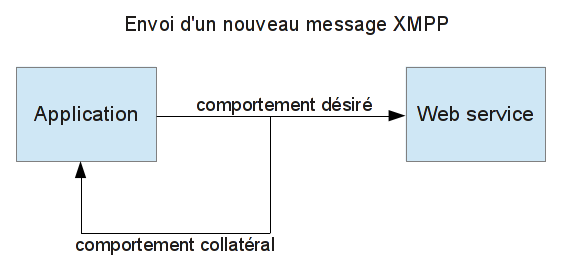
\includegraphics[width=12cm]{img/boucle-envoi-xmpp.png}
	\caption{Création d'une boucle lors de l'envoi d'un message XMPP}
	\label{boucle-envoi-xmpp}
\end{figure}

Comme le montre l'image \ref{boucle-envoi-xmpp}, une boucle se crée. Dans les faits, elle ne causera jamais de problème 
néanmoins c'est un comportement qui n'était pas désiré et qu'on aurait souhaitait évité.
\\\\
Deuxièmement, l'utilisation de GTalk était problématique. L'impossibilité de gérer finement GTalk fait que
tous les messages que nous envoyons, que ce soit depuis le téléphone ou bien depuis le site web étaient
aussi redirigés vers les outils utilisant GTalk.
\\
En pratique, cela impliquait de recevoir des messages au format JSon sur plusieurs lieux indésirables.

\begin{figure}[!h]
	\center
	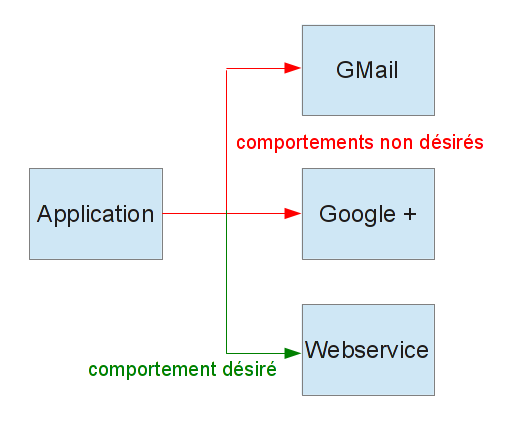
\includegraphics[width=10cm]{img/broadcast-xmpp.png}
	\caption{destinataires lors d'un envoi d'un message XMPP}
	\label{broadcast-xmpp}
\end{figure}

Comme le montre le schéma \ref{broadcast-xmpp}, lors de l'envoi d'un message XMPP originellement destiné uniquement
à une application ou au webservice, c'est tous l'environnement qui reçoit et affiche le nouveaux messages.
Le résultat est montré dans l'image \ref{message-xmpp-json-gmail}, un message XMPP au format JSon. 
	
\begin{figure}[!h]
	\center
	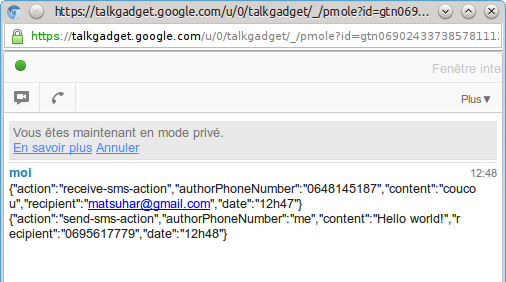
\includegraphics[width=10cm]{img/message-xmpp-json-gmail.png}
	\caption{message XMPP au format JSON reçu avec GTalk}
	\label{message-xmpp-json-gmail}
\end{figure}

\paragraph{Limite des SMS}
~~\\



%%%%%%%%%%%%%%%%%%%%%%%%%%%%%%%%%%%%%%%%%%%%%%%%%%%%%%%%%%%%%%%%%%%%%%%%%%%%%%%%%%%%%%%%%%%%%%%%%%%%
%%%%%%%%%%%%%%%%%%%%%%%%%%%%%%%%%%%%%%%%%%%%%%%%%%%%%%%%%%%%%%%%%%%%%%%%%%%%%%%%%%%%%%%%%%%%%%%%%%%%
%%%%%%%%%%%%%%%%%%%%%%%%%%%%%%%%%%%%%%%%%%%%%%%%%%%%%%%%%%%%%%%%%%%%%%%%%%%%%%%%%%%%%%%%%%%%%%%%%%%%

\subsection{iOS}

- envoi du SMS : n'apparait pas dans les messages : ajout à la main dans la BDD ?



Impossible de lire les contacts...
\\
